\documentclass[12pt]{article}

\usepackage{sbc-template}
\usepackage{graphicx,url}

%\usepackage[brazil]{babel}   
\usepackage[utf8]{inputenc}  
\usepackage{pgfgantt} % For Gantt charts
\usepackage{enumitem}

\sloppy

\title{Analysis of Communities formed on Youtube Comment Sections}

\author{Thiago Amado Costa\inst{1}, Humberto Torres Marques Neto\inst{1}}


\address{ICEI – Pontifícia Universidade Católica de Minas Gerais (PUC-MG)\\
    Belo Horizonte, Minas Gerais - Brasil \email{thiago.amado@sga.pucminas.br, humberto@sga.pucminas.br} }

\begin{document}

\maketitle

\begin{abstract}
    YouTube is the largest video streaming platform on the web, attracting billions of users 
    daily who watch and engage with content through comments. 
    A significant portion of these users consists of children and teenagers, who frequently interact 
    with one another in the comment sections, forming active communities. 
    However, these communities can also experience negative interactions between users, 
    including instances of online bullying and hate speech.
    To explore these communities, the YouTube Data API v3 was used to collect comments 
    from videos produced by creators targeting this demographic. 
    Topic modeling and sentiment analysis were then applied to further explore the 
    content and dynamics within these communities.
\end{abstract}

\section{Introduction}
% >> Descrição de motivações
% >> Problema escolhido e objetivos

% - youtube
% - kids, teenagers 
% - brasil 
% - bullying, 
% - comentarios, comunidades 

Youtube has grown exponentially since its launch in 2005. With billions of users, it is now the 
largest video streaming platform on the web, and and a major source of online entertainment content. 
As mentioned by \cite{app13064044}, many children and teenagers use the platform as an alternative to 
traditional entertainment sources, such as television, with the majority of their 
browsing time spent on YouTube.

One of the ways kids and teenagers interact on the platform is through the comment section. 
This feature allows users to share their thoughts on the video, the content creator, 
or even other commenters. These interactions can form online communities, and the analysis of these
communities can provide valuable insights into the dynamics of user interaction, providing a deeper 
understanding of the platform's social ecosystem.

The study by \cite{app13064044} showed that many of the current developments focus on identifying
innapropriate content targeting young children, with textual, video and audio analysis. 
Unfortunately, there is limited research focused on analysing the communities formed by kids and 
teenagers. 

Therefore, this study aims to analyze the community structures that emerge within the comment 
sections of Youtube creatore who create content aimed at children and teenagers, 
as well as the content of the comments themselves.

\section{Related Work}
% YOUTUBE 123 + Brazil + KIDS

% Comunidade
A social network community can be defined as a set of members of that specific network that interact
with each other, similar to real-world communities but in a online environment.
These online communities are shaped based on how users interact on each platform, and the analysis
of such communities can uncover hidden relationships between users and how they engage (\cite{nooribakhsh2024community}).

A recent research by \cite{kirdemir2023} uses community analysis to investigate coordinated 
inauthentic campaigns on YouTube, focusing on characterizing suspicious behaviors through a 
multi-step analysis of engagement trends and co-commenter networks. These co-commenter networks are
built by connecting two commenters if they commented on the same video.
By analysing these co-commenter networks and channel engagement trends, they were able to identify
patterns indicative of manipulation, such as increasing views paired with decreasing subscribers, 
and highlight channels exhibiting coordinated 
commenting behaviors. 

\cite{shajari2023} follows the methodology of \cite{kirdemir2023} to
explore the problematic behaviors of commenters on YouTube, specifically focusing on "commenter mobs" 
that manipulate engagement metrics to distort public perception. 
By analyzing 20 targeted channels through social network analysis, the research fills gaps in 
understanding how suspicious commenter activities boost engagement, which has been insufficiently 
addressed in prior literature. Employing a co-commenter network model and clustering techniques, 
the study identifies distinct groups with varying levels of suspiciousness and highlights collusion 
among commenters across channels. Key findings reveal central figures driving discussions and 
coordinated efforts to amplify specific narratives, suggesting these channels significantly contribute 
to the spread of misinformation. 

\cite{hussain2018analyzing} investigates disinformation tactics used on a specific conspiracy theory 
channel, distinguishing its approach by focusing on user engagement patterns rather 
than just spam detection. Data was collected using the YouTube Data API, monitoring metrics like views, 
likes, dislikes, and comments, revealing patterns indicative of potential manipulation. 
The analysis identified two commenter groups, peripheral and core, with the second group exhibiting higher 
instances of inorganic behaviors. A co-commenter network analysis revealed clusters around specific 
conspiracy topics and identified bot-like and spam actions. 

% Polarizacao / Topic Modeling
\cite{shekar2021} investigates the prevalence and nature of abusive comments on YouTube, 
particularly focusing on the impact of hate speech on users, especially teenagers. 
Utilizing exploratory data analysis and topic modeling, the research aims to identify patterns of 
abuse and the most affected content creators by manually labeling a custom dataset due to the lack 
of publicly available resources. Data was collected from selected YouTube celebrities using the 
YouTube Data API, and a thorough cleaning process resulted in a Document Term Matrix for analysis. 
The study employed Latent Dirichlet Allocation (LDA) for topic modeling and sentiment analysis using 
the TextBlob library to assess the emotional tone of comments. Findings revealed that certain 
YouTubers received significantly harsher comments, with varying sentiment levels indicating the 
need for interventions to protect young creators from severe online harassment. 
The study concludes by recommending measures such as disabling comments on particularly abused 
videos and emphasizes the importance of understanding the dynamics of cyberbullying.

\section{Methodology}

This study uses a similar methodology as previous works. It consists of a data collection phase, 
a community analysis phase, and a content analysis phase.

\subsection{Data Collection}

Initially, the YouTube Data API v3 was used to gather comprehensive channel metadata for each 
specific YouTuber. Subsequently, we retrieve the IDs and titles of 50 videos from each channel. 
Finally, we construct the YouTuber's comments dataset by aggregating all comments and replies 
associated with each video, as well as the author information and the number of likes of each comment. 
For this, 10 different popular youtube channels were chosen, with content varying from gaming and 
vlogging, with the number of subscribers ranging from 8 million to 46 million. The number of comments
collected per channel ranges approximately 11,000 to 43,000.


\subsection{Community Analysis}

To analyze the communities that emerge within each YouTuber's comment section, the datasets constructed 
in the previous phase is used to construct the co-commenter networks. Each commenter is connected to
another if they commented on the same video, and the weight of the edge is increased if they commented
on more than one video together. To maintain only the stronger connections, we filtered out co-commenters
who commented on less than 10 videos together, as done by \cite{shajari2023} and \cite{kirdemir2023}. 

To identify the communities of each co-commenter network the Louvain Algorithm was used. This 
agorithm was chosen because of its high efficiency and performance on real-world networks
without ground truth, as shown by \cite{YOU2020104822}

Following the method developed by \cite{kirdemir2023}, a set of metrics were computed 
for each co-commenter network, including average degree, number of nodes and edges, average coefficient,
modularity, coverage, the number of communities identified with the Louvain Algorithm. Graph clique 
metrics were also computed, including the number of maximal cliques that have at least five members, 
average clique size, median clique size, average degree of clique members, average clustering coefficient
of clique members. To discover the similarities between the chosen channels, these metrics were used
with KMeans and Hierarchical Clustering, along with Principal Component Analysis to reduce the complexity
while maintaining important features.

\subsection{Content Analysis}

To further understand user behaviour, we implement
topic modeling and sentiment analysis. For the topic modeling phase, we employ the BERTopic model 
(\cite{bertopic2022}), while the sentiment analysis is conducted using the multilingual 
XLM-roBERTa-base model (\cite{barbieri-etal-2022-xlm}). 
Initially, the comments are processed and cleaned, masking user handles to preserve anonymity,
removing emojis, links and stopwords
Then, topic modeling is utilized to extract themes associated with the communities identified in the 
previous phase. Finally, the sentiment analysis model evaluates the polarity of the content, 
offering deeper insights into the emotional tone of the discussions and facilitating a more 
comprehensive analysis of the communities.

\section{Results}

In this section, the results are shown and analyzed.

\subsection{Community Analysis}

Considering that a modularity value above 0.3 is a good indicator of significant
community structures in a network \cite{PhysRevE.70.066111}, The Louvain Algorithm successfully 
identified communities in all of the youtubers's co-commenter networks, with the lowest value beeing
0.52 and the highest beeing 0.90. 

The KMeans and Hierarchical Clustering methods were applied with the community metrics described. 
Both methods identified 4 distinct clusters, as can be seen in Figure ~\ref{fig:kmeans_hierarchical}.
Then, each cluster identified is analyzed separately.

\begin{figure*}[ht]
    \centering
    \begin{minipage}{0.44\textwidth}
        \centering
        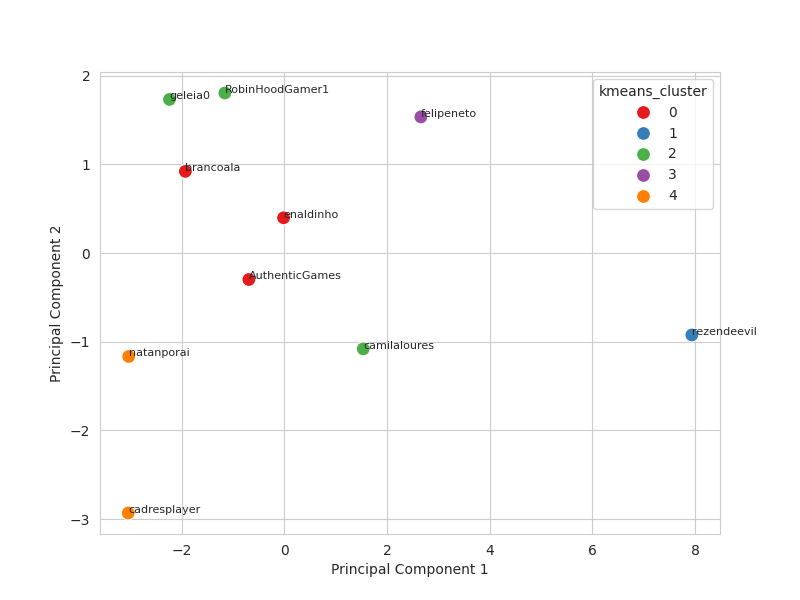
\includegraphics[keepaspectratio,width=\textwidth]{./imgs/KMeans_PCA.png}
    \end{minipage}%
    \hspace{0.0001\textwidth} 
    \begin{minipage}{0.45\textwidth}
        \centering
        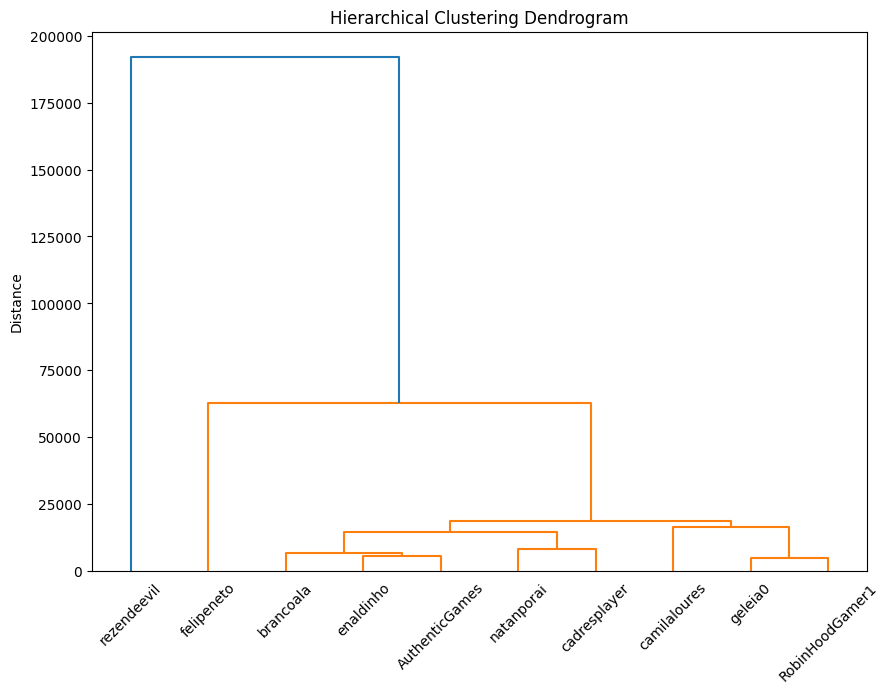
\includegraphics[keepaspectratio,width=\textwidth]{./imgs/Hierarchical_clustering.png}
    \end{minipage}
    \caption{KMeans and Hierarchical Clustering}
    \label{fig:kmeans_hierarchical}
\end{figure*}


The most distinguishable channels are on clusters 1 (Rezendeevil) and 3 (Felipe Neto). 
Both youtubers had a very high number of nodes and edges, with Rezendeevil's network having 13.808 
nodes and 149.033 edges, and Felipe Neto having 24.987 nodes and 125.165 edges.
The youtuber Rezendeevil, who has the lowest modularity also had the highest 
average degree of 21.5, number of maximal cliques and average clique size.
Similarly, youtuber Felipe Neto had a lower modularity score of 0.64, a high number of maximal cliques,
and a high average degree of 10.
This indicates that both youtubers have high interconnected and engaged communities. The higher average
degree indicates that Rezendeevil's followers are more engaged than Felipe Neto's, while the higher
modularity score shows that Felipe Neto's community structure is more distinct.
This can be seen through Figure~\ref{fig:rezendeevil_comm} and Figure ~\ref{fig:felipeneto_comm}, 
with each community colored. 

% The youtuber with the highest modularity score, Geleia, has many smaller and distinct communities, 
% as can be seen in Figure~\ref{fig:geleia_comm}

\begin{figure*}[t!]
    \centering
    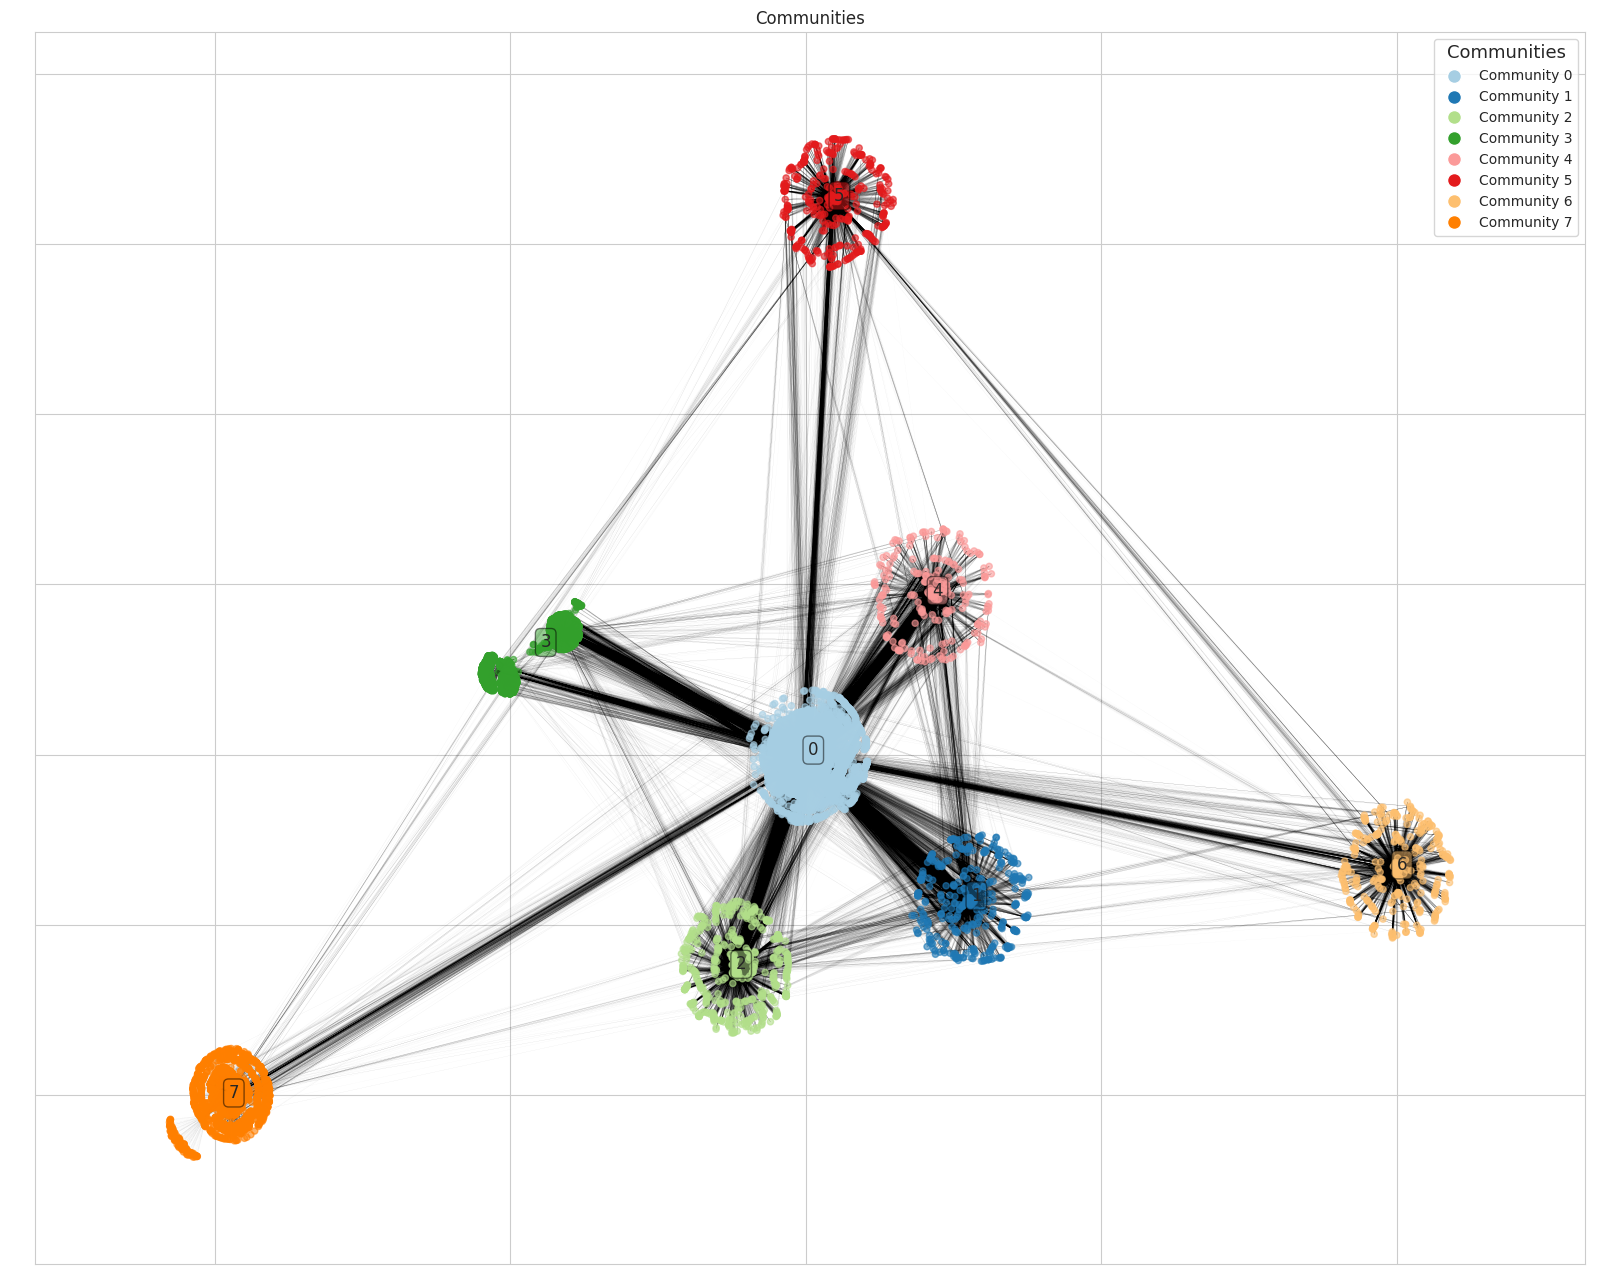
\includegraphics[keepaspectratio,width=0.9\textwidth]{./imgs/rezendeevil/communities.png}
    \caption[width=\textwidth]{Rezendeevil's Communities}
    \label{fig:rezendeevil_comm}
\end{figure*}

\begin{figure*}[t!]
    \centering
    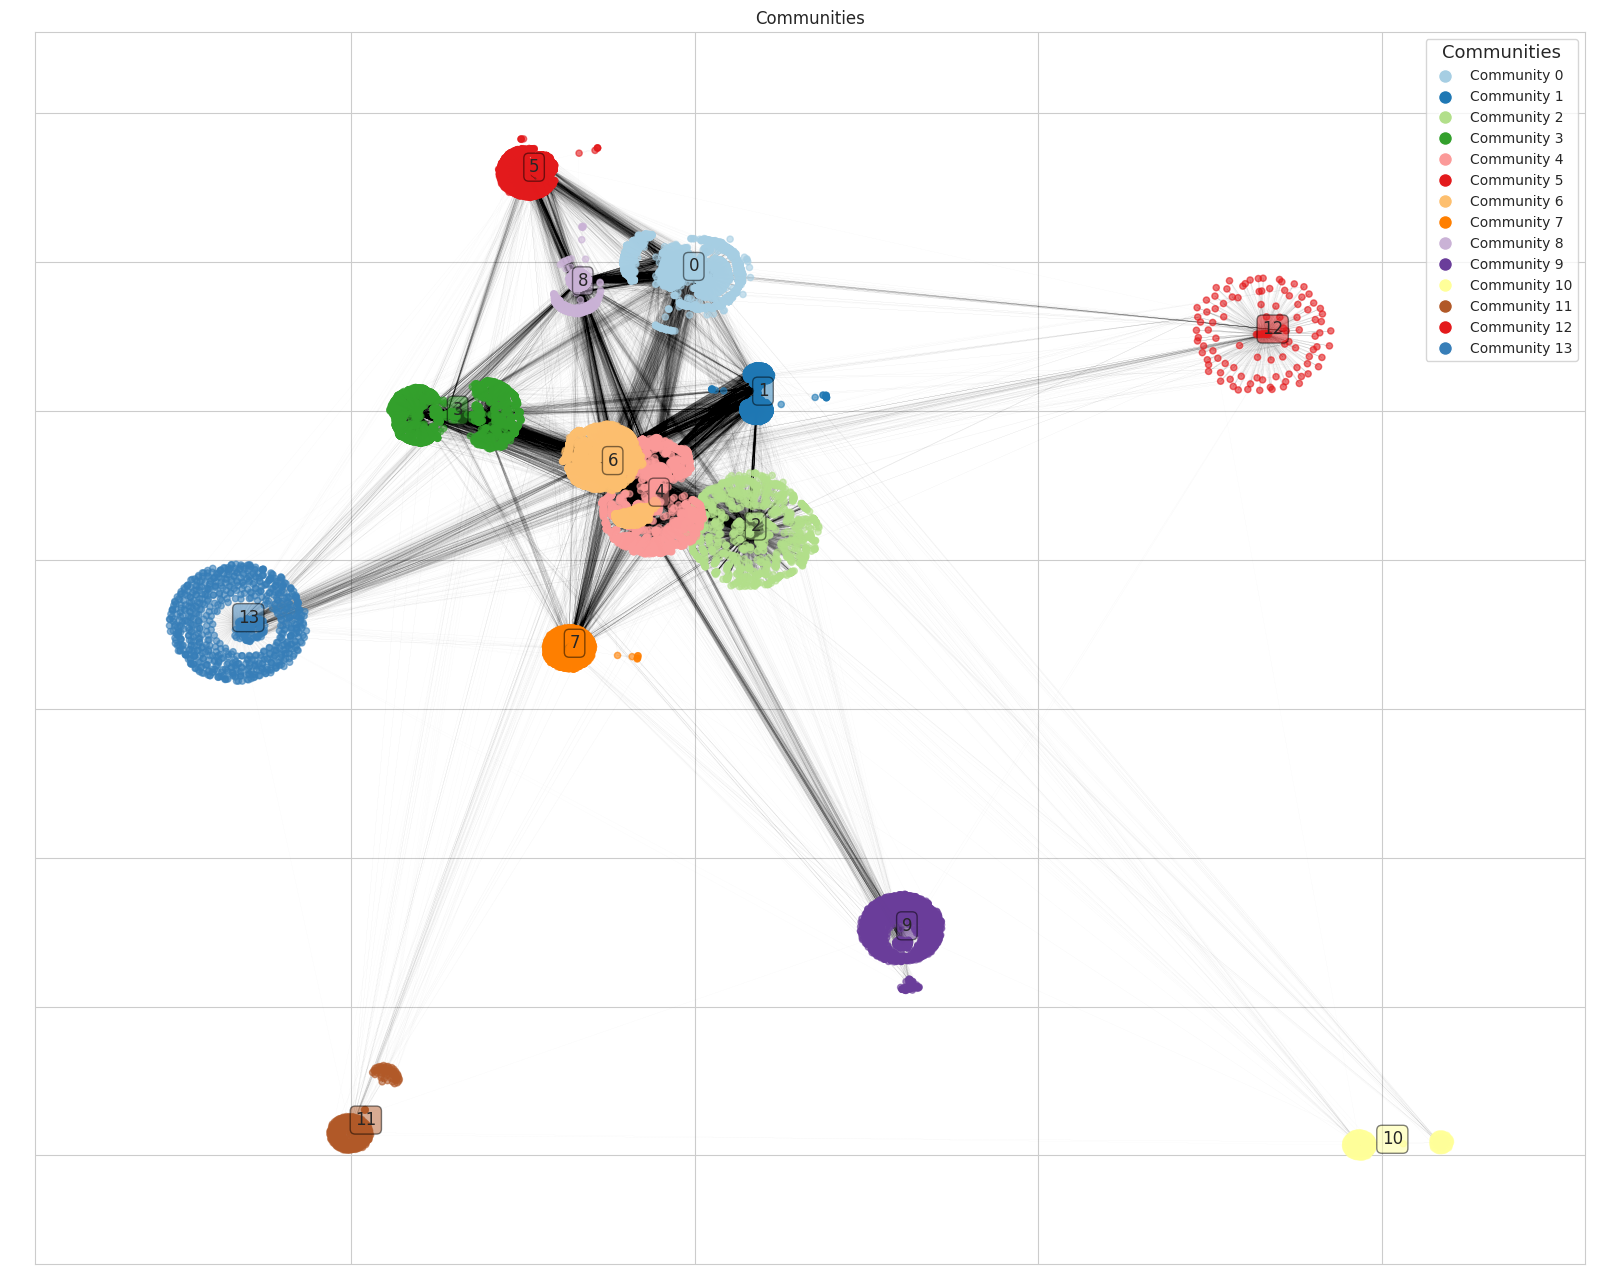
\includegraphics[keepaspectratio,width=0.9\textwidth]{./imgs/felipeneto/communities.png}
    \caption[width=\textwidth]{Felipe Neto's Communities}
    \label{fig:felipeneto_comm}
\end{figure*}


Cluster 0 has the most similar network structures. All three youtuber's networks have around 11.500
nodes and around 30.000 edges. Youtubers Enaldinho and AuthenticGames have modularity scores of
0.75 and 0.72 respectively, and Brancoala has the modularity score of 0.86. They also have similar
numbers of maximal cliques and average clique sizes.


\bibliographystyle{sbc}
\bibliography{sbc-template}

\end{document}
